%!TEX root = ../main.tex

\chapter{Clustering} % (fold)
\label{cha:clustering}

Il clustering può essere considerato il più importante problema di \textbf{apprendimento non supervisionato} in quanto trova innumerevoli applicazioni in svariati campi del sapere. L’obiettivo che si pone è organizzare dati non classificati in gruppi, i cui membri sono simili per un qualche criterio. Un \textbf{cluster} è quindi una collezione di oggetti che sono simili tra di loro, e dissimili dagli oggetti appartenenti ad altri cluster. Formalmente:

\begin{mydef}[Problema del clustering]
	Dati $n$ oggetti e una matrice di similarità $n \times n$ lo scopo è partizionare gli inputs in gruppi massimalmente omogenei (i.e \textbf{clusters}).
\end{mydef}

Il criterio di similarità che deve essere fornito per poter fare un clustering dei dati può essere visto come una funzione $\phi$ che dati due oggetti ritorna la loro similarità. Questa misura è \emph{simmetrica} se per una qualunque coppia di oggetti $(a, b)$ abbiamo che $\phi(a, b) = \phi(b, a)$ altrimenti è \emph{asimmetrica}.\\

\begin{figure}[h!]
	\centering
	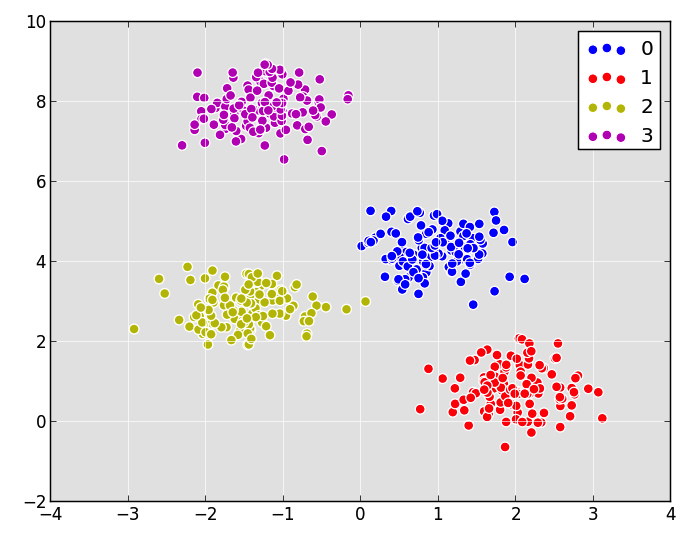
\includegraphics[width=8cm]{images/clustering.png}
	\caption{Esempio di clustering}\label{fig:clusters}
\end{figure}

In questo esempio è possibile identificare tre cluster nei quali possono essere suddivisi i dati e il criterio di similarità usato è la \emph{distanza}, quindi due oggetti fanno parte di uno stesso cluster solo se sono sufficientemente vicini tra di loro. 

\newpage

Questo tipo di clustering è detto \emph{distance-based}, ovvero basato sulla distanza. In generale, a seconda del tipo di input il problema del partizionamento si divide in:
\begin{enumerate}
	\item \textbf{feature-based:} gli oggetti sono rappresentati come vettori di caratteristiche. Nella letteratura l'algoritmo più noto è il \emph{k-means};
	\item \textbf{pairwise:} le proprietà degli oggetti sono meglio descritte in termini di \emph{similarità/dissimilarità} tra di essi. In questo caso l'input è determinato da una matrice di affinità che indica la similarità tra tutte le coppie di oggetti. Si tratta quindi di un approccio più generale rispetto al primo.
\end{enumerate}

Non sempre è facile ed intuitivo trovare un raggruppamento per i dati, come invece lo era per l’esempio visto, in quanto è difficile stabilire cosa costituisce un “buon clustering” e cosa no. In generale si può affermare che un cluster deve soddisfare i seguenti criteri:
\begin{itemize}
	\item \textbf{criterio interno}: tutti gli oggetti all'\emph{interno} di un cluster devono essere il più possibile simili tra loro;
	\item \textbf{criterio esterno}: tutti gli oggetti all'\emph{esterno} di un cluster devono essre il più possibile dissimili rispetto a quelli contenuti al suo interno.
\end{itemize}

Nelle sezioni seguenti saranno presentate alcune metodologie di clustering e ci si concentrerà, infine, sull'utilizzo della teoria dei giochi per risolvere il problema.


\newpage

\section{K-Means} % (fold)
\label{sec:k_means}
K-Means è probabilmente il più famoso algoritmo di partizionamento feature-based. Dato un insieme di osservazioni $\{x^{(1)},\dots,x^{(n)} \}$ dove $x_i$ è un vettore m-dimensionale, lo scopo dell'algortimo è partizionare l'insieme in $k$ insiemi $k \leq n$ il più possibile coesi tra loro (problema del clustering).\\

L'algoritmo seleziona a caso $k$ prototipi, rappresentanti il proprio gruppo di appartenzenza, idealmente il centro del cluster. Formalmente si ha un insieme di vettori:
\begin{align*}
	\mu_j, \text{ dove } j = 1, \dots, k
\end{align*}
L'obiettivo ora consiste nel raggruppare le osservazioni e reimpostare i vettori $\mu_j$ in modo tale che la somma del quadrato delle distanze da un punto al proprio centroide $\mu_j$ sia minima. In termini matematici si tratta di minimizzare la seguente funzione:
\begin{align}
	\min_{\{\mu_1, \dots, \mu_k\}} \sum_{i=1}^n \sum_{j=i}^k r_{ij} \| x_i - \mu_j \|^2\label{eq:j}
\end{align}
dove $r_{ij}$ è un operatore binario $r_{ij} \in \{ 0, 1 \}$. In fase di inizializzazione, si scelgono $k$ punti casuali come centri e in seguito si esegue una procedura iterativa per minimizzare \eqref{eq:j}. Ogni iterazione si compone di \textbf{due} fasi: nella prima fase (\emph{Expectation-Step}) si minimizza rispetto a $r_{ij}$ mantenendo $\mu_j$ fisso, mentre nella seconda fase (\emph{Maximization-Step}) si minimizza rispetto a $\mu_j$ mantenendo $r_{ij}$ fisso. Formalmente, nella fase E, il calcolo di $r_{ij}$ è dato da:
\begin{align*}
	r_{ij} =
	\begin{cases}
		1, &\text{ se }j = argmin_j \| x_i - \mu_j \|^2 \\
		0, &\text{ altrimenti}
	\end{cases}
\end{align*}
Intuitivamente si assegna l’osservazione $x_i$ al gruppo con $\mu_j$ più vicino.

\newpage

Nella seconda fase $\mu_k$ è dato da:

\begin{align*}
	\mu_j = \frac{\displaystyle\sum_i r_{ij} x_i}{\displaystyle\sum_i r_{ij}}
\end{align*}

Ovvero, si cerca di “spostare” al centro del cluster il prototipo $\mu_j$ come la media di tutti i punti $x_i$ assegnati al cluster $k$. Queste due fasi si ripetono fino a quando non c'è più alcuna variazione negli assegnamenti o quando un numero massimo di iterazioni è raggiunto. Infatti, trattandosi di un problema NP-Difficile non è dato sapere a priori se l'algoritmo converga oppure no.

\begin{figure}[h!]
	\centering
	\subfigure{
	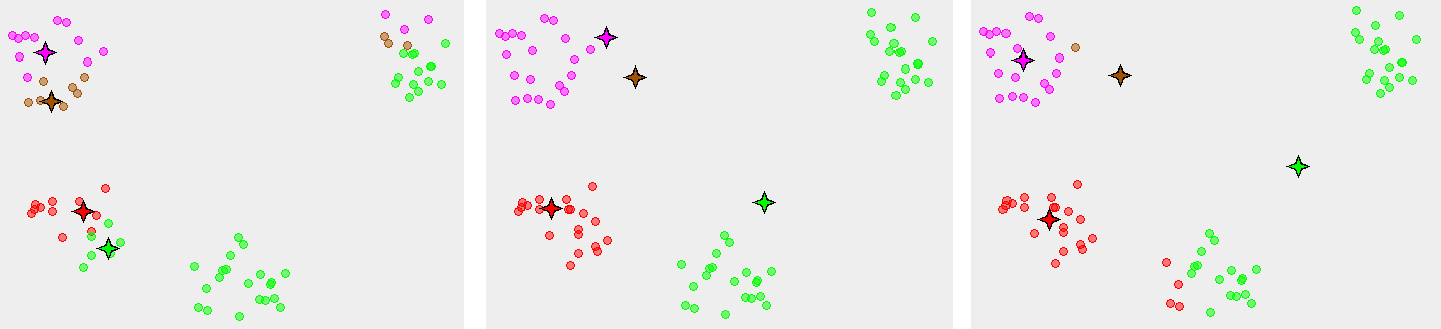
\includegraphics[width=12cm]{images/kmeans}
	}
	\subfigure{
	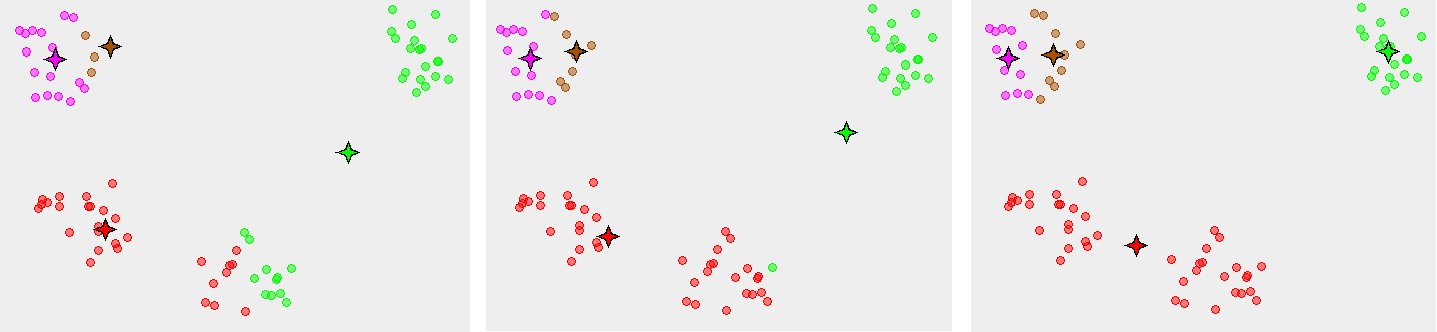
\includegraphics[width=12cm]{images/kmeans2}
	}
	\caption[Convergenza in K-means]{Esempio sulla convergenza (dopo 5 iterazioni) a un minimo locale dell'algoritmo k-means}
\end{figure}

% section k_means (end)


\section{Normalized Cut} % (fold)
\label{sec:normalized_cut}
A differenza del k-means l'algoritmo presentato in questa sezione è basato sulla teoria dei grafi e trova ampio utilizzo nella \emph{segmentazione delle immagini}, un problema analogo al clustering.
L'algoritmo \emph{normalized cut} “taglia” l'immagine utilizzando tecniche della \textbf{teoria spettrale} dei grafi. Un buon taglio divide pixel che sono dissimili tra loro. Per trovare un buon partizionamento l'algoritmo segue i seguenti passi:
\begin{enumerate}
	\item Si costruisce un grafo di similarità $G=(V, E, w)$ in cui ogni nodo rappresenta un pixel dell'immagine e il peso su ciascun arco rappresenta una misura di similarità (intensità, colore ecc..) tra ciascun pixel.
	\item Si calola il Laplaciano normalizzato definito come:
	\begin{align}
		L = D ^ {- 1 / 2} (D - A) D ^ {- 1 / 2}
	\end{align}
	dove $A$ è la matrice di adiacenza pesata e $D$ è la matrice dei gradi così definita:
	\begin{align}
		d_{i,j}:=
		\begin{cases} 
			\deg(v_i) & \mbox{if}\ i = j \\
			0 & \mbox{otherwise}
		\end{cases}
	\end{align}
	Si calcolano gli autovettori del Laplaciano normalizzato:
	\begin{align}
		L x = \lambda x
	\end{align}
	
	\item Utilizzando il segno nel secondo autovettore più piccolo (il primo è un vettore nullo) si segmenta l'immagine in due parti.

	\item La procedura si ripete ricorsivamente fino a quando si ottiene il numero desideerato di segmenti.
\end{enumerate}

L'algoritmo nella pratica si è dimostrato abbastanza efficace tuttavia il calcolo degli autovettori è un problema computazionalmente costoso: $O(n^3)$ dove $n$ è il numero di pixel. Tuttavia è possibile velocizzare l'algoritmo sfruttando il fatto che la matrice è sparsa (i valori sono quasi tutti pari a zero) ed abbassare la complessità a $O(n \sqrt{n})$\\

\begin{figure}[h!]
	\centering
	\subfigure[$original$]
	{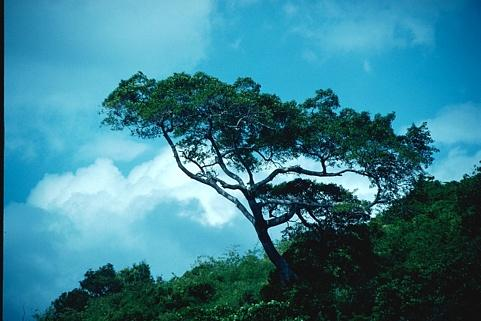
\includegraphics[width=3cm]{images/0.jpg}}
	\subfigure[$k = 2$]
	{
\includegraphics[width=3cm]{images/1.png}}
	\subfigure[$k = 3$]
	{
\includegraphics[width=3cm]{images/2.png}}
	\subfigure[$k = 4$]
	{
\includegraphics[width=3cm]{images/3.png}}
	\caption{Esempio di segmentazione ottenuta con NCUT.}
\end{figure}


% section normalized_cut (end)

\newpage


\section{Insiemi dominanti} % (fold)

Il concetto di insieme dominante nasce dallo studio sulla formulazione continua del problema della cricca massima (vedi Sezione~\ref{sec:problema_della_cricca_massima}). L'insieme dominante, infatti, non è altro che una clique di un grafo nel caso in cui gli archi siano pesati, ovvero insiemi di vertici che hanno alta omogeneità interna e alta disomogeneità verso l'esterno.\\

In questo contesto i dati sono, dunque, rappresentati da un grafo non orientato $G = (V, E , w)$ dove $V = \{ 1, \dots, n \}$ è l'insieme dei vertici, $E\subseteq V \times V$ l'insieme degli archi e $w : E \rightarrow \mathbb{R}_+$ è la funzione dei pesi positiva. I vertici rappresentano i datapoints, gli archi le relazioni tra essi e i pesi rispecchiano la similarità tra coppie di vertici connessi.\\

Come di consueto, il grafo è rappresentato con la sua matrice di adiacenza pesata $A$, che è la matrice simmetrica $n \times n$ dove $A = a_{ij}$ è definito nel seguente modo:
\begin{align*}
	a_{ij} =
	\begin{cases}
		w(i, j), &\text{ if }(i, j) \in E\\
		0, &\text{ otherwise }
	\end{cases}
\end{align*}

Si consideri $S \subseteq V$ un insieme non vuoto di vertici $i \in S$. Si introduce il concetto di \textbf{grado pesato medio} di $i$ rispetto ad $S$ definito come:\\

\begin{minipage}{.5\textwidth}
	\begin{align*}
		awdeg_S(i) = \frac{1}{|S|}\sum_{j \in S} a_{ij}
	\end{align*}
	E nel caso in cui $j \not\in S$:
	\begin{align*}
		\phi_S(i,j) = a_{ij} - awdeg_S(i)
	\end{align*}
\end{minipage}
\begin{minipage}{.5\textwidth}
	\begin{tikzpicture}[node distance=2cm]
		\fill [gray!20] (-1, 0) ellipse  (2cm and 3cm);
		\node at (-1, 3.4) {$S$};
		\node[Node] (1) at (0,0) {$i$};
		\node[Node, left of=1] (2) {};
		\node[Node, above of=2] (3) {};
		\node[Node, below of=2] (4) {};
		\node[Node, right=2cm of 1] (0) {$j$};
		\path
		(1) edge (2) edge (3) edge (4) edge[above] node{$a_{ij}$} (0)
		;
		\end{tikzpicture}\\
	\end{minipage}

	Intuitivamente $\phi_S(i, j)$ misura la similarità tra il nodo $j$ e il nodo $i$ rispetto alla similarità media tra il nodo $i$ e i suoi vicini in $S$

	\newpage

	Il peso di $i$ rispetto ad $S$ è quindi definito come:
	\begin{align*}
		w_S(i) =
		\begin{cases}
			1, &\text{ if }|S|=1\\
			\displaystyle\sum_{j \in S \setminus \{i\}} \phi_{S \setminus \{i\}} (i, j) \cdot w_{S \setminus \{i\}}(j) &\text{ otherwise}
		\end{cases}
	\end{align*}
	Si tratta di una definizione ricorsiva e permette di assegnare un peso (similarità relativa) ad ogni vertice.
	E il peso totale di $S$ è:

	\begin{minipage}{.5\textwidth}
		\begin{align*}
			W(S) = \sum_{i \in S} w_S(i)
		\end{align*}
	\end{minipage}
	\begin{minipage}{.5\textwidth}
		\begin{tikzpicture}[node distance=2cm]
			\fill[gray!20] (0, 0) circle  (3cm);
			\fill[gray!40, rotate=-45] (-0.5, 0) ellipse  (2cm and 2.5cm);
			\node[Node] (1) at (0, 0) {$j$};
			\node[Node, above of=1] (2) {};
			\node[Node, below left of=1] (3) {};
			\node[Node, above of=3] (4) {};
			\node[Node, below right=1.5cm of 1] (5) {$i$};
			\node[Node, above right of=1] (6) {};
			\path (1) edge (2) edge (3) edge (5) edge (6)
			(3) edge (4)
			;
		
			\node (1) at (0, 3.4) {$S$};
			\node (1) at (0, -2.3) {$S \setminus \{i\}$};
		\end{tikzpicture}
		\\
	\end{minipage}

	Intuitivamente $w_S(i)$ ci dà la misura di similarità complessiva tra il nodo $i$ e i vertici $S \setminus \{i\}$ rispetto alla similarità complessiva di ciascun vertice in $S \setminus \{i\}$. Si considerino i seguenti grafi.

	\begin{figure}[h!]
		\centering
		\subfigure[$W_{\{1,2,3,4\}(1)} < 0$]{
		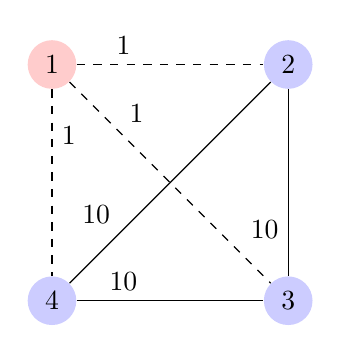
\begin{tikzpicture}[node distance=3cm]
			\node[circle,fill=red!20] (1) at (0,1.5) {1};
			\node[circle,fill=blue!20, right of=1] (2) {2};
			\node[circle,fill=blue!20, below of=1] (4){4};
			\node[circle,fill=blue!20, below of=2] (3) {3};

			\foreach \from / \to in {1/2,1/3,1/4}
			\path (\from) edge[dashed, near start, auto] node{$1$} (\to);

			\foreach \from / \to in {4/2,4/3,3/2}
			\path (\from) edge[near start, auto] node{$10$} (\to);
		\end{tikzpicture}
		}
		\qquad\qquad
		\subfigure[$W_{\{5,6,7,8\}(5)} > 0$]{
		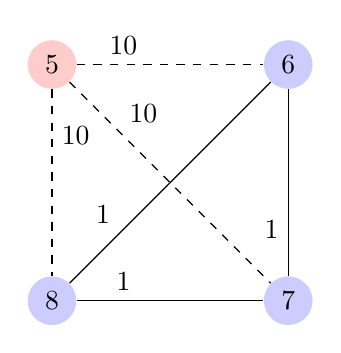
\begin{tikzpicture}[node distance=3cm]
			\node[circle,fill=red!20] (1) at (0,1.5) {5};
			\node[circle,fill=blue!20, right of=1] (2) {6};
			\node[circle,fill=blue!20, below of=1] (4){8};
			\node[circle,fill=blue!20, below of=2] (3) {7};

			\foreach \from / \to in {1/2,1/3,1/4}
			\path (\from) edge[dashed, near start, auto] node{$10$} (\to);

			\foreach \from / \to in {4/2,4/3,3/2}
			\path (\from) edge[near start, auto] node{$1$} (\to);
		\end{tikzpicture}
		}
		\caption[Insiemi dominanti e similarità]{Rappresentazione della similarità: i nodi $\{2,3,4\}$ sono altamente simili tra loro. Se si tenta di aggiungere il vertice 1 che è dissimile dalla similarità interna dell'insieme $\{2,3,4\}$ allora la similarità complessiva del nuovo insieme $\{1,2,3,4\}$ diminuisce i.e. $W_{\{1,2,3,4\}}(1) < 0$. Nel secondo caso il vertice 5 è altamente similare ai nodi $\{6,7,8\}$ di conseguenza aggiungendolo all'insieme la similarità complessiva aumenta i.e. $W_{\{5,6,7,8\}}(5) > 0$.}
	\end{figure}

	\newpage

	È stata dunque definita una misura che descrive cosa comporta (in termini di similarità) l'aggiunta o la rimozione di un nodo. Questo porta alla definizione di \emph{insiemi dominanti}.

	\begin{mydef}[Insieme Dominante]
		Un sottoinsieme di vertici non vuoto $S \subseteq V$ tale che $W(T) > 0$ per ogni insieme non vuoto $T \subseteq S$ è detto \textbf{dominante} se:
		\begin{enumerate}
			\item $W_S(i) > 0, \forall i \in S$ (omogeneità interna)
			\item $W_{S \cup \{i\}}(i) < 0, \forall i \not\in S$ (disomogeneità esterna)
		\end{enumerate}
	\end{mydef}
	L'insieme dominante è dunque un insieme di vertici massimalmente coesi tra loro e questa definizione corrisponde con quella di cluster.

	\begin{figure}[h!]
		\centering
	
		\begin{tikzpicture}[node distance=3cm]
			\node[circle,fill=blue!20] (1) at (0,0) {1};
		
			\node[circle,fill=blue!20, below left of=1] (2) {2};
			\node[circle,fill=blue!20, below right of=1] (3) {3};
        
			\node[circle,fill=blue!20, below of=2] (4) {4};
			\node[circle,fill=blue!20, below of=3] (5) {5};

			\foreach \from / \to / \label in {1/2/10,1/3/15,1/4/60,1/5/70}
			\path (\from) edge[near start] node{$\label$} (\to);
			
			\foreach \from / \to / \label in {2/4/25,2/5/20}
			\path (\from) edge[near start] node{$\label$} (\to);

			\foreach \from / \to / \label in {3/4/25,3/5/90}
			\path (\from) edge[near start] node{$\label$} (\to);

			\path (4) edge[auto] node{5} (5);
			\path (2) edge[auto] node{20} (3);

			\begin{pgfonlayer}{background}    % select the background layer
				\fill[gray!20] plot coordinates {(1) (3) (5)};
			\end{pgfonlayer}

		\end{tikzpicture}
		\caption{L'insieme $\{1,3,5\}$ è dominante.}
	\end{figure}

	Quando la matrice di affinità è binaria 0/1 allora l'insieme dominante coincide con la cricca massimale (stretta) in un grafo (vedi Sezione~\ref{sec:problema_della_cricca_massima}).\\

	\newpage

	\subsection{Insiemi dominanti e ottimi locali} % (fold)
	\label{sub:insiemi_dominanti_e_ottimi_locali}
	In questa sezione sarà mostrato come la teoria di Nash possa essere utilizzata per risolvere in modo approssimato la ricerca di insieme dominanti.\\

	Dato un grafo pesato $G = (V, E, w)$ e la sua matrice di adiacenza pesata $A$, si consideri il seguente programma quadratico standard:
	\begin{align*}
		&\text{maximize } f(x) = x^T A x\\
		&\text{subject to } x \in \Delta
	\end{align*}
	dove $\Delta$ è il simplesso standard su $R^n$. Si introduce il seguente teorema:

	\begin{thm}
		Se $S$ è un sottoinsieme dominante di vertici, allora il suo vettore caratteristico pesato $x^S$ definito come:
		\begin{align*}
			x^S_i = 
			\begin{cases}
				\frac{W_S(i)}{W(S)}, &\text{ se }i \in S\\
				0 &\text{ altrimenti}
			\end{cases}
		\end{align*}
		è un massimizzatore locale stretto di $f$ in $\Delta$.
	
		Al contrario se $x^*$ è un massimizzatore locale stretto di $f$ in $\Delta$ allora il suo supporto:
		\begin{align*}
			\sigma = \sigma(x^*) = \{ i \in V : x^*_i \neq 0 \}
		\end{align*}
		è un insieme dominante a condizione che $W_{\sigma \cup \{i\}} \neq 0$ per ogni $i \not\in \sigma$. 
	\end{thm}
	Dove la condizione $W_{\sigma \cup \{i\}} \neq 0$ è un tecnicismo dovuto alla presenza di soluzioni spurie, ovvero soluzioni che non ammettono vettore caratteristico pesato. Si tratta di una generalizzazione del teorema di Motzkin Strauss.\\

	Ora che è stata fornita una caratterizzazione di insieme dominante è possibile utilizzare una qualunque tecnica di ottimizzazione quadratica per risolvere il problema (ad esempio la discesa del gradiente). Tuttavia le dinamiche di replicazione (vedi Sezione~\ref{sec:teoria_dei_giochi_evoluzionistici}) si sono rivelate particolarmente adatte per affrontare questo problema. È stato infatti dimostrato il seguente teorema:

	\begin{thm}[Torsello, Rota Bulò, Pelillo 2006]
		Strategie evolutionary stable (ESS) di un problema di clustering con matrice di affinità $A$ sono in corrispondenza uno-a-uno con gli insiemi dominanti.
	\end{thm}

	\newpage

	Quindi sia $A$ la matrice di adiacenza del grafo di similarità. Si pone:
	\begin{align*}
		W = A (= W^T \geq 0)
	\end{align*}
	Allora un sistema di replicazione con matrice di payoff $W$ partendo da uno stato iniziale arbitrario convergerà, per il principio di selezione naturale, a un massimizzatore della funzione $f(x) = x^T A x$ nel simplesso standard. Questo corrisponderà a un insieme dominante in un grafo, ovvero ad un cluster di vertici. Quindi la ricerca di dominant sets di un grafo pesato e non orientato $G$, corrisponde a trovare equilibri di Nash asintoticamente stabili e le dinamiche di replicazione sono un ottimo strumento a disposizione per perseguire questo scopo.\\

	La teoria dei giochi evoluzionistici opera in uno scenario in cui coppie di individui sono scelti ripetutamente a caso da una grande popolazione per competere in un gioco a due giocatori. A differenza della teoria dei giochi classica, i giocatori non si comportano razionalmente ma sono pre-programmati a un certo pattern comportamentale o una strategia mista. Col passare del tempo il principio di selezione naturale inciderà sulla distribuzione dei comportamenti.\\

	Ad esempio si supponga di volere separare lo sfondo in un'immagine dagli elementi in primo piano. Nel gioco evoluzionistico ogni giocatore è pre-programmato a selezionare con una certa probabilità un elemento (un pixel) dall'immagine. In questo contesto la selezione naturale porterà giocatori che adottano strategie migliori (payoff più alto) ad espandersi, mentre quelli che adottano strategie peggiori ad estinguirsi. Nel caso descritto, ci si aspetta che la selezione naturale porti all'estinzione i giocatori che selezionano lo sfondo, per poi convergere a una popolazione che seleziona solo gli elementi in primo piano.\\

	Concludendo le caratteristiche principali che rendono questo approccio preferibile rispetto ad altri sono le seguenti:
	\begin{enumerate}
		\item Non richiede alcuna rappresentazione dei dati ovvero che gli elementi debbano essere rappresentato come punti in uno spazio vettoriale;
		\item assenza di assunzioni circa la struttura della matrice di affinità: è stato dimostrato che l'approccio funziona anche nel caso di funzioni di similarità asimmetriche o negative;
		\item non è necessaria alcuna conoscenza a priori circa il numero di clusters;
		\item permette l'estrazione di cluster sovrapposti.
	\end{enumerate}

	% subsection insiemi_dominanti_e_ottimi_locali (end)
	% section insiemi_dominanti (end)
	
	
	\section{Problema di etichettatura} % (fold)
	\label{sec:problema_di_etichettatura}
	In un tipico labelling (consistent) problem si hanno:
	\begin{itemize}
		\item $n$ oggetti $B= \{b_1, \dots, b_n\}$;
		\item $m$ etichette (labels) $\Lambda = \{\lambda_1, \dots, \lambda_m\}$.
	\end{itemize} 
	Lo scopo è assegnare a ciascun oggetto in $B$ un'etichetta in $\Lambda$.\\
	
	I legami tra oggetti ed etichette sono espressi attraverso una matrice 4-dimensionale $n^2 \times m^2$ di coefficienti di compatibilità reali $R = \{r_{ij}(\lambda, \mu)\}$: la componente $r_{ij}(\lambda, \mu)$ misura la forza di compatibilità tra le due ipotesi “$\lambda$ è sull'oggetto $b_i$” e “$\mu$ è sull'oggetto $b_j$”. Alti valori significano alta compatibilità mentre bassi valori indicano incompatibilità.\\
	
	Sia $p_i(\lambda)$ il grado di confidenza dell'ipotesi “l'etichetta $\lambda$ è sull'oggetto $b_i$”. Allora la distribuzione di probabilità delle etichette su un oggetto $b_i$ è un vettore $m$-dimensionale:
	\begin{align*}
		\bar{p}_i = (p_1 (\lambda_1), \dots, p_n(\lambda_m))^T
	\end{align*}
	con $p_i(\lambda) \geq 0$ e $\sum_\lambda p_i(\lambda) = 1$. Mettendo insieme i $\bar{p}_i$ si ottiene un \emph{assegnamento pesato delle etichette} per gli oggetti in $B$ denotato come $\bar{p}$, una matrice $n \times m$. Lo spazio degli assegnamenti pesati delle etichette è un insieme lineare convesso in $\mathbb{R}^{nm}$:
	\begin{align*}
		\mathcal{K} = \underbrace{\Delta \times \dots \times \Delta}_\textrm{$m$ times}
	\end{align*}
	dove $\Delta$ è il simplesso standard in $\mathbb{R}^n$. Ogni vertice in $\mathcal{K}$ rappresenta un assegnamento non ambiguo ovvero che assegna esattamente un'etichetta a ciascun oggetto. L'insiemi di questi labelling sarà denotato da $\mathcal{K}^*$.\\
	
	Si consideri un labelling $\bar{p} \in \mathcal{K}$. La \textbf{consistenza} di un oggetto misura il grado di confidenza tra l'ipotesi “$b_i$ è etichettato con $\lambda$” ed il contesto. Questo concetto può essere quantificato attraverso la seguente funzione di supporto lineare:
	\begin{align*}
		q_i(\lambda; \bar{p}) = \sum_j \sum_\mu r_{ij} (\lambda, \mu) p_j(\mu)
	\end{align*}
	
	\newpage
	
	Sia $p \in \mathcal{K}^*$ e sia $\lambda(i)$ l'etichetta assegnata a $b_i$ da $\bar{p}$ (i.e. $p_i(\lambda(i) = 1)$). Allora si dice che $\bar{p}$ è consistente se e solo se l'etichetta assegnata a ciascun oggetto riceve il più alto supporto da quell'oggetto. Questo corrisponde ad avere:
	\begin{align*}
		q_i(\lambda; \bar{p}) \leq q_i(\lambda(i); \bar{p})
	\end{align*}
	per ogni $i$ e $\lambda$. Applicando lo stesso ragionamento l'assegnamento pesato $\bar{p} \in \mathcal{K}$ è \emph{consistente} se:
	\begin{align*}
		\sum_\lambda v_i(\lambda)q_i(\lambda; \bar{p}) \leq \sum_\lambda p_i(\lambda) q_i(\lambda; \bar{p})
	\end{align*}
	per ogni $i = 1, \dots, n$ e $\bar{v} \in \mathcal{K}$. Inoltre se la disuguaglianza è stretta per ogni $\bar{v} \neq \bar{p}$, allora $\bar{p}$ è detto \emph{strettamente consistente}.\\
	
	Hummel e Zucker hanno dimostrato che se la matrice di compatibilità è simmetrica $r_{ij}(\lambda, \mu) = r_{ji}(\mu, \lambda)$ allora una condizione sufficiente affinché $\bar{p}$ sia consistente corrisponde a un minimo locale della seguente funzione energia che misura la (in)consistenza tra labelling:
	\begin{align*}
		A(\bar{p}) = \sum_{i, \lambda} \sum_{j, \mu} r_{ij}(\lambda, \mu) p_i(\lambda) p_j(\mu)
	\end{align*}
	
	Un processo \textbf{relaxation labelling} prende in input un assegnamento di etichette iniziale $\bar{p}^{(0)} \in \mathcal{K}$ e lo aggiusta iterativamente tenendo conto del modello di compatibilità utilizzando la seguente regola di aggiornamento:
	\begin{align}
		p_i^{(t + 1)}(\lambda) = \frac{p_i^{(t)}(\lambda) q_i^{(t)} (\lambda)}{\displaystyle\sum_\mu p_i^{(t)}(\mu) q_i^{(t)} (\mu)}\label{eq:relax}
	\end{align}
	Purchè la matrice di compatibilità sia non-negativa. Il processo evolve fino a quando non viene raggiunto un punto fisso ovvero quando $\bar{p}^{(t + 1)} = \bar{p}^(t)$. Nella pratica è solito fermare il processo quando la distanza tra due etichettamenti successivi è sotto una certa soglia oppure dopo un certo numero di iterazioni. Queste tecniche sono particolarmente utilizzate nel campo della visione artificiale.
	
	\newpage
	
	\subsection{Relaxation labelling e teoria dei giochi} % (fold)
	\label{sub:relaxation_labelling_e_teoria_dei_giochi}
	È possibile formulare un processo relaxation labelling in termini di teoria dei giochi. In questa formulazione:
	\begin{itemize}
		\item i giocatori sono gli oggetti;
		\item le etichette sono le strategie pure;
		\item gli assegnamenti pesati corrispondono alle strategia miste;
		\item la matrice di compatibilità è la matrice di payoff.
	\end{itemize}
	Pertanto un equilibrio di Nash corrisponde a un labelling consistente e un equilibrio di Nash stretto a un labelling consistente stretto. Inoltre la regola di aggiornamento~\eqref{eq:relax} corrisponde alla dinamica di replicazione utilizzata nella teoria dei giochi evoluzionistici (vedi Sezione~\ref{sec:teoria_dei_giochi_evoluzionistici}).\\
	
	Si tratta di un \textbf{polimatrix game}: un gioco non-cooperativo succinto in cui per ogni coppia di giocatori $i, j$ esiste una matrice di payoff che indica una componente del guadagno di un giocatore $i$. Il payoff totale per tale giocatore è la somma delle componenti. Formalmente:
	\begin{itemize}
		\item Ci sono $n$ giocatori con $m$ strategie;
		\item Per ogni coppia $i, j$ di giocatori c'è una matrice di payoff $A^{ij}$ di dimensione $m \times m$;
		\item Il payoff del giocatore $i$ per una certa combinazione di strategie $s_1, \dots, s_n$ è dato da:
		\begin{align*}
			\mu_i(s_1,\dots,s_n) = \sum_{j \neq i} A^{ij}_{s_i s_j}
		\end{align*}
	\end{itemize}
	Il numero di payoff per rappresentare questo gioco è $O(n^2, m^2)$. Il problema di trovare un equilibrio di Nash è PPAD-completo.
	% subsection relaxation_labelling_e_teoria_dei_giochi (end)
	% section problema_di_etichettatura (end)
	
	
	\newpage
	
	
	\section{Trasduzione di grafi} % (fold)
	\label{sec:trasduzione_di_grafi}
	La trasduzione di grafi è una popolare classe di tecniche di apprendimento semi-supervisionato che mirano a stimare la funzione di classificazione definita su un grafo in cui alcuni nodi (datapoints) sono classificati e altri no. L'idea generale consiste nel propogare in maniera consistente l'informazione appresa nei nodi etichettati a quelli non etichettati.\\
	
	Formalmente dato un insieme di datapoints $\mathcal{D} = \{\mathcal{D}_\ell, \mathcal{D}_u\}$ dove:
	\begin{itemize}
		\item $\mathcal{D}_\ell = \{(x_1, y_1), \dots, (x_\ell, y_\ell\}$ sono gli oggetti etichettati;
		\item $\mathcal{D}_u = \{x_{\ell + 1}, \dots, x_n\}$ sono gli oggetti non etichettati.
	\end{itemize}
	Le relazioni tra questi oggetti sono date da un grafo pesato non orientato $G=(V,E)$ dove i vertici rappresentano gli oggetti e gli archi misurano la similarità tra le coppie di nodi. Nel caso speciale in cui il grafo non sia pesato (la matrice di adiacenza è binaria) la presenza di un arco tra due nodi $i, j$ indica una similarità perfetta. In questo caso un cluster è dunque una componente connessa del grafo.\\
	
	\begin{figure}[h!]
	    \centering
	    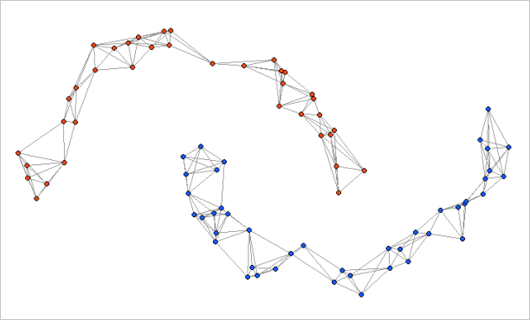
\includegraphics[width=12cm]{images/transduction}
		\caption{Apprendimento trasduttivo su un grafo non pesato.}
	\end{figure}
	
	\newpage
	
	Sia $A = a_{ij}$ la matrice di adiacenza binaria allora il problema della trasduzione su grafi non pesati può essere formalizzato come un \emph{problema di soddisfacimento di vincoli} (CSP) definito su un insieme di variabili $V = \{v_1, \dots, v_n\}$ i cui valori appartengono ai seguenti domini:
	\begin{align*}
		D_{v_i} =
		\begin{cases}
			\{y_i\}, &\text{ per ogni }1 \leq i \leq \ell\\
			Y, &\text{ per ogni }\ell + 1 \leq i \leq n\\
		\end{cases}
	\end{align*}
	e soggetto ai seguenti vincoli binari:
	\begin{align*}
		\forall i, j: \text{se } a_{ij} = 1, \text{allora } v_i = v_j
	\end{align*}
	Ad esempio in un problema a due classi i vincoli sono così definiti:
	\begin{align*}
		R_{ij} = 
		\begin{pmatrix}
			1 & 0 \\
			0 & 1
		\end{pmatrix}
	\end{align*}
	Una soluzione ad un CSP è un assegnamento di valori alle variabili che soddisfi tutti i vincoli e corrisponde ad un'etichettatura consistente per i nodi non classificati.\\
	
	È possibile risolvere un CSP con la teoria dei giochi. Si consideri il seguente gioco chiamato “\emph{graph transduction game}” (GTG). Si assuma che ogni giocatore $i \in \mathcal{I}$ corrisponda a un particolare punto nel dataset $\mathcal{D} = \{d_1, \dots, d_n \}$ e che possa scegliere una strategia nell'insieme $S_i = \{ 1, \dots, c\}$ in cui ciascuna strategia rappresenta l'ipotesi di appartenenza ad una certa classe e $c$ è il numero totale di classi.\\
	
	Per definizione del problema i giocatori sono divisi in due gruppi disgiunti:
	\begin{enumerate}
		\item \textbf{giocatori etichettati}: consapevoli della loro classe di appartenenza e denotati dall'insieme $\mathcal{I}_\ell = \{\mathcal{I}_{\ell \mid 1}, \dots, \mathcal{I}_{\ell \mid c}\}$ in cui ogni sottoinsieme $\mathcal{I}_{\ell \mid k}$ indica i giocatori che giocano sempre le loro $k$ strategie pure.
		\item \textbf{giocatori non etichettati}: $\mathcal{I}_\mu$.
	\end{enumerate}
	Ovviamente solo i giocatori non etichettati andranno a competere nel GTG in quanto i giocatori etichettati sono vincolati a giocare una strategia definita.
	
	\newpage
	
	Si suppone che in questo gioco ogni arco nel grafo rappresenti un gioco a due giocatori e quindi il payoff di ciascun giocatore è la somma dei payoff guadagnati ad ogni giocata con uno dei suoi vicini. Formalmente dato un profilo strategico misto $x = (x_1, \dots, x_n)$ la funzione di payoff di un giocatore $i \in \mathcal{I}$ è:
	\begin{align*}
		\mu_i(x) = \sum_{j=1}^n x_i^T A_{ij} x_j
	\end{align*}
	dove $A_{ij}$ è la \emph{matrice di payoff parziale} tra i giocatori $i$ e $j$. Il gioco è quindi governato dalla seguente funzione payoff:
	\begin{align*}
		\mu_i(x) = \sum_{j \in \mathcal{I}_\mu} x_i^T A_{ij} x_j + \sum_{k=1}^c \sum_{j \in \mathcal{I}_{\mathcal{D} \mid k}} x_i^T (A_{ij})_k
	\end{align*}
	Rimane ora da definire la matrice di payoff parziale. Data la matrice pesata $W = (w_{ij})$ allora la matrice di payoff parziale tra due giocatori è data da $A_{ij} = w_{ij} \times I_c$ dove $I_c$ è la matrice identità di dimensione $c$. Si noti che se la matrice di payoff parziale è rappresentata a blocchi $A = (A_{ij})$, allora la matrice $A$ è data dal prodotto di Kronecker $A = I_c \otimes W$. Ad esempio in un problema a tre classi la matrice di payoff parziale $A_{ij}$ è nella seguente forma:
	\begin{align*}
		A_{ij} =
		\begin{pmatrix}
			w_{ij} & 0 & 0 \\
			0 & w_{ij} & 0 \\
			0 & 0 & w_{ij} 
		\end{pmatrix}
	\end{align*}
	Si noti infine che nel caso di matrici di similarità binarie, allora le matrici di payoff parziale coincidono con le matrici di compatibilità definite nel CSP. Inoltre, se sono ammesse solo strategie pure allora il GTG si riduce al CSP. In questo caso in un equilibrio di Nash puro i giocatori nel vicinato giocano la stessa strategia pura con lo scopo di ottenere il payoff massimo contro i vicini. Tale equilibrio di Nash corrisponde alla soluzione del CSP se ne esiste una altrimenti il CSP è insoddisfabile e quindi il GTG non ammette equilibri di Nash.
	
% section trasduzione_di_grafi (end)
% chapter clustering (end)





















